\subsubsection{Przywracanie grafu do początkowego rozmiaru wraz z ulepszeniem podziału}

Kolejną częścią algorytmu jest faza przywracania grafu do początkowej wielkości.
Tej fazie towarzyszy poprawianie podziału, które polega na zmniejszaniu długości granic oraz na
wyrównywaniu wielkości pól pomiędzy obszarami.
Ten etap nadaje podziałowi ostateczny kształt.
W tym celu zaimplementowana została zmodyfikowana heurystyka Helpful Sets (HS) \cite{10.1007/3-540-44842-X_6}.
Efekt jej działania widoczny jest na rysunku \ref{im:refinement}.
\vspace{2mm}
\begin{figure}[h]
\centering
\begin{subfigure}{.5\textwidth}
    \centering
    \fbox{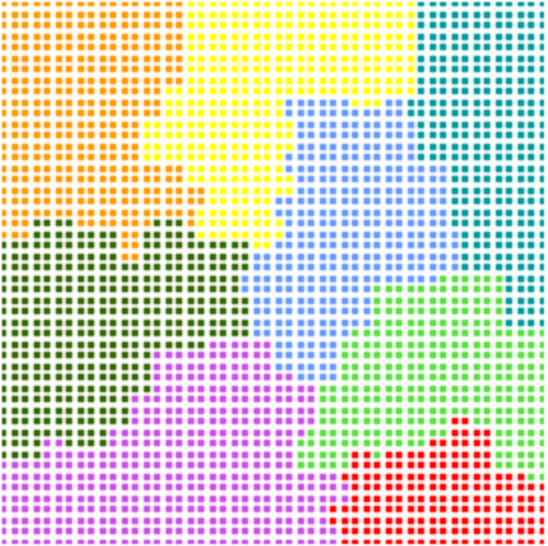
\includegraphics[width=0.4\textwidth]{images/refinement/1}}
    \caption[short]{po algorytmie LAM}
\end{subfigure}%
\begin{subfigure}{.5\textwidth}
    \centering
    \fbox{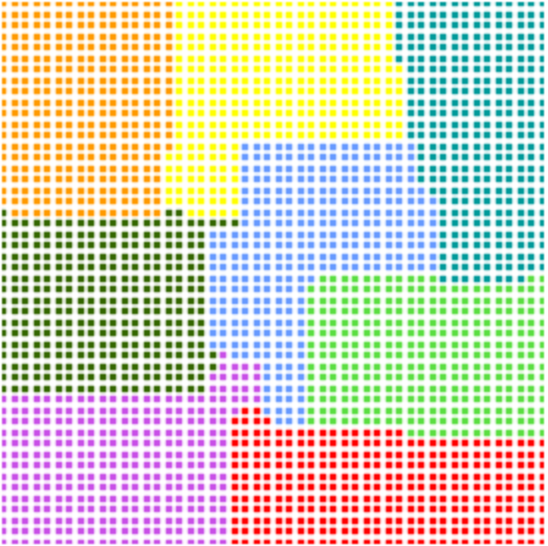
\includegraphics[width=0.4\textwidth]{images/refinement/2}}
    \caption[short]{po fazie ulepszania}
\end{subfigure}
\caption{Obrazek (a) przedstawia partycjonowanie siatki (a) samym algorytmem LAM.
Obrazek (b) przedstawia ulepszenie podziału z obrazka (a). Zmniejszona została długość granic oraz wyrównane zostały pola.}
\label{im:refinement}
\end{figure}


Etap pierwszy to heurystyka HS do poprawiania podziału.
Jest oparta na wyszukiwaniu lokalnym -
próbuje poprawić aktualny podział poprzez wielokrotne wprowadzanie lokalnych zmian.
Wierzchołki klasyfikowane są
pod kątem liczby krawędzi łączących je z wierzchołkami obszaru do którego należą (ang. internal edges) oraz z wierzchołkami
pozostałych obszarów (ang. external edges).
Wedle tej klasyfikacji wierzchołki przy granicach wymieniane są między obszarami.
Niech $A$ i $B$ będą partycjami na siatce.
Algorytm dzieli się na dwie fazy.
Pierwsza buduje zbiór wierzchołków $C$ na wierzchołkach partycji $A$, a następnie przenosi go z partycji $A$ do partycji $B$.
Wierzchołki są dobierane tak, aby zmniejszyć długość granicy między obszarami.
Druga faza to szukanie zbioru balansującego $D$.
Jest budowany na zbiorze $B$.
Jego celem jest zwrócenie zbioru wierzchołków o tej samej wielkości jak zbiór $C$ z partycji $B$ do partycji $A$,
przy jednoczesnym możliwym utrzymaniu ulepszenia w długości granicy po wcześniejszej fazie.
Zbiór $C$ nazywamy \texttt{k-helpful set}, natomiast zbiór $D$ nazywamy \texttt{balancing set}.
Po etapie ulepszenia granicy następuje etap drugi mający na celu wyrównywanie powierzchni pól.
Używając tej samej klasyfikacji, wierzchołki przy granicach przenoszone są z obszarów mniejszych do większych.
Te dwa etapy powtarzane są co jakiś czas podczas przywracania grafu do początkowej wielkości.
Najpierw więc pracują na grafie o mniejszej liczbie wierzchołków, gdzie każdy wierzchołek reprezentuje zbiór wierzchołków.
W ten sposób efektywnie przenoszone są duże obszary w formie pojedynczych wierzchołków o dużych wagach.
Im dalej w procesie przywracania grafu, tym algorytm pracuje na większym grafie z wierzchołkami o mniejszych wagach.
Podział jest już ulepszony w poprzednich wywołaniach więc może dokonywać bardziej lokalnych poprawek.
\newpage
\begin{pseudocode}
@\underline{PROCEDURE RestoreGraphWithPartitionsImprovements}@
  $number\_of\_restoration\_steps\_done$ $\leftarrow$ $0$
  $number\_of\_all\_reductions$ $\leftarrow$ $reductions$.$length$
  WHILE $number\_of\_all\_reductions$ $-$ $number\_of\_restoration\_steps\_done$ $>$ $0$
    $reduction$ $=$ $reductions$.$pop()$
    RestoreReduction$(reduction)$
    $number\_of\_restoration\_steps\_done$ $\leftarrow$ $number\_of\_restoration\_steps\_done$ $+$ $1$
    IF $number\_of\_restoration\_steps\_done$ $/$ $number\_of\_all\_reductions$ $>$ $0.9$ AND
       floor$(number\_of\_all\_reductions$ mod $($$number\_of\_all\_reductions$ $\cdot$ $0.03))$ $==$ $0$
      ImprovePartitioning
    ENDIF
  ENDWHILE
  ImprovePartitioning
  WHILE there are any indivisible areas:
    area $\leftarrow$ pop one of them
    RestoreReduction(area)
  ENDWHILE
\end{pseudocode}
\vspace{-8mm}
\captionof{listing}{Algorytm przedstawia główną procedurę optymalizującą długość granic.}
\label{code:main_impr_procedure}
\vspace{4mm}
Na algorytmie \ref{code:main_impr_procedure}
przedstawiona jest główna procedura odpowiedzialna za przywrócenie grafu do
początkowej wielkości wraz z wprowadzaniem optymalizacji granic.
Autorzy artykułu \cite{1364754}, na podstawie którego stworzona została niniejsza praca, wyspecyfikowali, że
do optymalizacji granic używany jest algorytm HelpfulSets, który
wywoływany jest wielokrotnie na różnych etapach przywracania grafu.
Nie było natomiast informacji jak często oraz w jakich stadiach przywracania grafu wywoływany jest algorytm.
W związku z powyższym zaproponowałem wyżej opisane rozwiązanie.
Dodatkową modyfikacją algorytmu przywracania grafu było również uwzględnienie obszarów niepodzielnych.
Pierwsza pętla WHILE (linia $4$) odpowiedzialna jest za przywrócenie zwykłych
redukcji, to znaczy tych, które zostały stworzone przez algorytm LAM oraz wprowadzenie ulepszeń.
Inne redukcje to te, które wykonywane są na obszarach niepodzielnych zaraz po
algorytmie, który zamienia obrazek przedstawiający siatkę na graf.
Redukcje te przywracane są na samym końcu, po przeprowadzeniu optymalizacji granic.

Procedura \texttt{ImprovePartitioning} za każdym razem aktualizuje informacje o sąsiadujących obszarach, ponieważ
te mogą ulec zmianie na skutek kolejnych wywołań algorytmu, a następnie iteruje po wszystkich parach sąsiadujących obszarów i wywołuje
dla nich procedurę \texttt{HelpfulSet}.
Pseudokod procedury \texttt{HelpfulSet} został przedstawiony na algorytmie \ref{code:helpful_sets}.
Jak wynika z kodu (linia $8$) proces optymalizacji długości granic oraz pól obszarów zaczyna się dopiero,
gdy graf przywrócony jest do początkowej wielkości przynajmniej w $90\%$.
Tą wartością można manipulować dowolnie, jednak powinna być ona wysoka.
W momencie, kiedy pozwolimy algorytmowi optymalizować bardzo zredukowane grafy, to przesuwane na raz będą bardzo
duże pule wierzchołków.
Algorytm do optymalizacji granic został stworzony do wprowadzania małych, lokalnych zmiany, a nie przesuwania dużych obszarów.
Dlatego więc przy optymalizowaniu zredukowanych grafów niszczy podział, zamiast go poprawiać.
Efektem tego jest powstawanie obszarów podzielonych na dwie części.
Zjawisko to przedstawione jest na rysunku \ref{im:noises} i będzie dokładnej opisane w dalszych częściach pracy.
W linii $9$ widzimy także, że optymalizacja przeprowadzana jest co pewną liczbę przywróconych redukcji.
Bowiem przywrócenie jednej redukcji, to zamiana jednego wierzchołka na dwa wierzchołki, które zastąpiła.
Jest więc to zmiana zbyt mała, żeby ponownie włączać optymalizację dla całego grafu.
Na podstawie przeprowadzonych prób można stwierdzić, że współczynniki powinny być ustawione tak, aby wywoływać
algorytm optymalizacji granic $5$-$10$ razy podczas przywracania grafu.
Takie wartości gwarantują dobry wynik przy niezbyt długim czasie wykonania.
Więcej wywołań niekoniecznie da lepszy rezultat.
Ta funkcjonalność została zaimplementowana przy użyciu operacji wyliczania reszty z dzielenia.
W linii $13$ następuje ostatnie wywołanie algorytmu optymalizacji granic, już na niemal całkowicie przywróconym grafie
(nie licząc obszarów niepodzielnych).
Ostatnim krokiem jest przywrócenie obszarów niepodzielnych, co dzieje się w drugiej pętli WHILE
w linii $14$.